
\section{Six Key Words}
Satellite image, Lake size scaling, Fractal dimension, Machine learning, General lake model (Carbon fluxes, Microbes). 
\section{Introduction}
The carbon flow is a crucial indicator for calculating the amount of carbon emissions. Several studies indicated that ponds and lakes, particularly those in forested areas or with thermokarst deposits in the Arctic or Tibet Plateau, are among those that produce the most carbon\citep{serikova2019high,holgerson2017gas,karlsson2021carbon}. A small pond would retain much carbon and release it into the air, according to \cite{holgerson2016large}. As \cite{cael2016size} reported, both the local and global lake views show that the lake size does not scale according to the power law. The \cite{mandelbrot1982fractal} provided a fractal theory that scaled the ponds differently. Hence, \cite{cael2016size} study of the lakes in Sweden and worldwide reveals a significant relationship between lake density and area. When the lakes shrink in size, the difference becomes apparent. In addition, the small shallow ponds tend to release carbon by active microbes decomposing sediment and primary producer consuming\citep{bartosiewicz2015greenhouse,colina2022role}. Large lakes may cover broad surface areas, but millions of smaller lakes with more active reactions would create and store more carbon than a single huge lake. Thus, there is a trend to research tiny lakes across the world that emit carbon.\\
In my proposal, the final ambition is to calculate the Total Carbon Emission from ponds which is equal to the Ponds Density X Carbon Emission rate (Samraat provide this hypothesis to me). In the first part, it is the ponds density that needs to be re-verified with the conclusion reported by \cite{cael2016size} by applying new data, general lake model(3.0) simulation \cite{hipsey2019general} and  Machine Learning method. The proposed research questions are listed below:\\
1.Compare with the result reported by \cite{cael2016size} with updated data and new ponds definition \citep{richardson2022functional} to verify whether the power-low would be fitted with data or not in small lakes. (under time change scale) \\
2.Whether the different variables of the lakes distribution (e.g. regions, latitude, altitude, land-use change etc.) will fit similarly to the results of \cite{cael2016size}'s study. \\
(Then, in the second part, the Carbon Emission rate affected by microbes from ponds will be researched if there is spare time.)




\section{Proposed Methods}

1. Data preparation and model training. Search for \cite{cael2016size}'s database and find if there is any new data and review the classification of ponds. Learn the GLM, with the physical parameters, to set the ponds' model. Search for \cite{richardson2022functional}'s database, and find the newest pond data and related variables.\\
2. Re-scaling ponds data but with more variables. If there is the newest global ponds data, do similar as \cite{cael2016size} do, compare the newest ponds' abundance with areas (but with a more accurate definition of ponds \citep{richardson2022functional}). The power-law test would be applied and followed with \cite{downing2009global}'s study. Besides, the Shoreline fractal dimension would be computed as \cite{cael2016size}'s method. The global ponds line vs power low simulated line would be compared under changed time. Then, according to \cite{verpoorter2014global} and \cite{richardson2022functional}, the description of their ponds database shows that various variables could be studied with ponds. For instance, the regions, the locations, the elevations etc. I will attempt to test all of them to see how the abundance vs area would be different with power low under different conditions.\\
3.Validation by satellite images and GLM(general lake model). The trained GLM model by machine learning would be applied to fit with the real ponds data and compared with power low to see the fitness of model simulation and further changes. Besides, the newest regional high resolutions satellite image may be processed by QGIS and output some local pond data to do the validation.
\\
Appendix 1. Apart from the restudying, the scaling lakes problems. The rest time would be spent researching the connections between carbon emissions, microbial biomass, and small lakes. Data from a different research study may be used to evaluate their association.


\section{Anticipated Outputs and Outcomes}
1. Test a relationship between lake area and lake density that is at least as good as \cite{cael2016size} results. The conclusion may state that worldwide ponds and small lakes follow similar criteria, but all different with the estimated power-law distribution. The different variables, such as changed time, regions and elevation would produce similar curve plots.
\\
Appendix 1. Find a link between those three variables on a quantitative and qualitative level, and maybe create a model to suit the local and global data.


\section{project Feasibility and Timeline}
\begin{figure}[H]
    \centering
    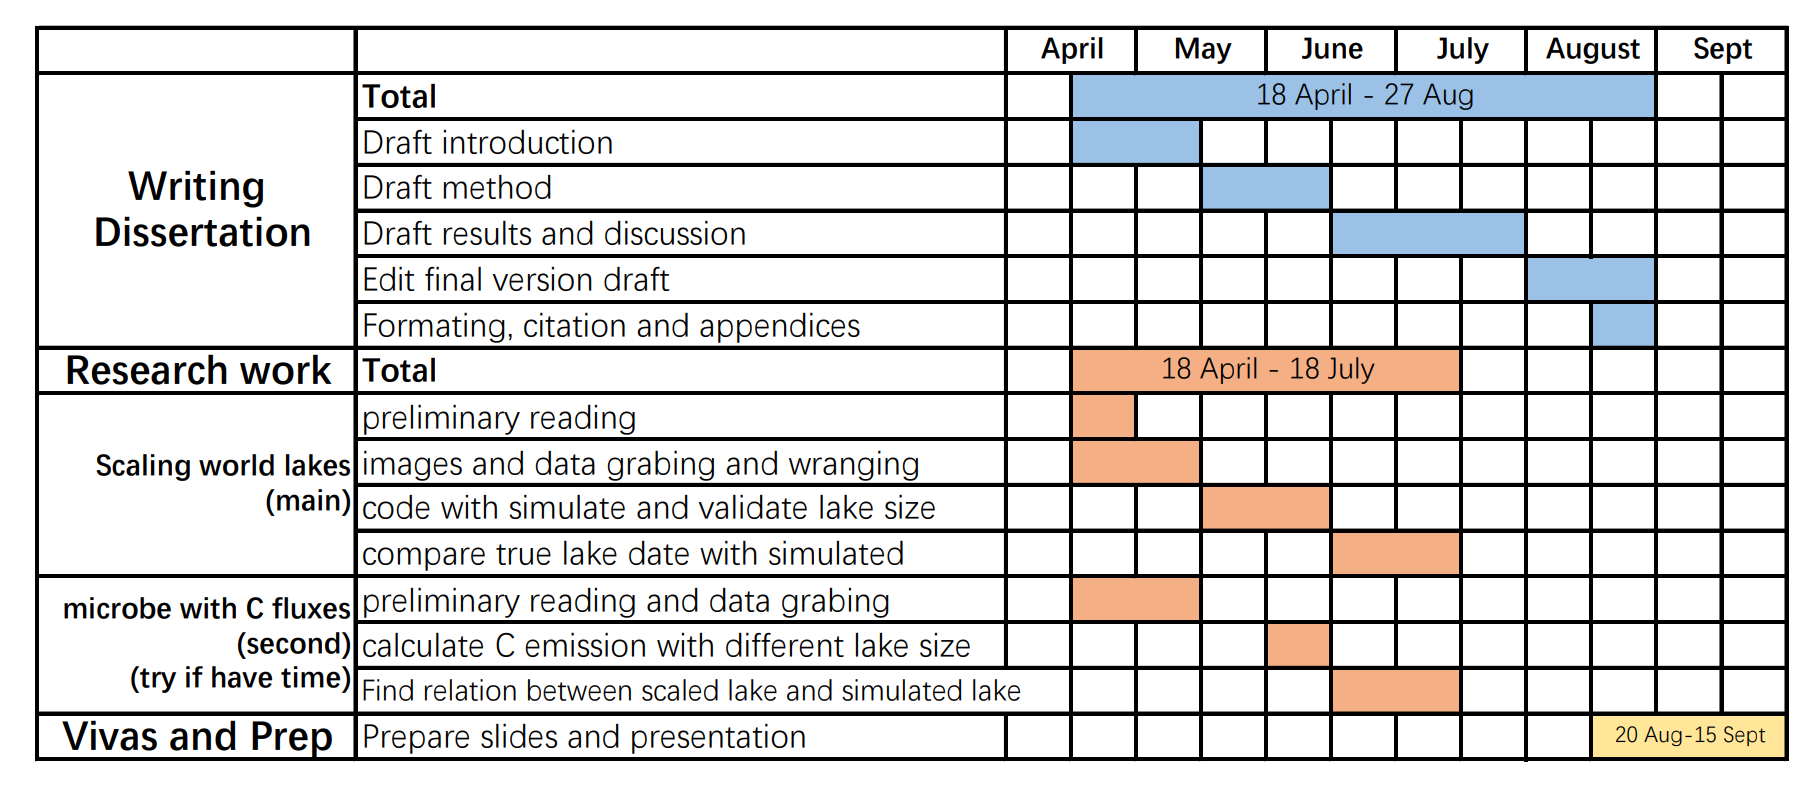
\includegraphics[scale=0.4]{introduction/Figure1.png}
    \caption{MSc Imperial Project}
    \label{Fig.1}
\end{figure}

\section{Budget}
Other items that might enhance project completion are presented in Figure 2. Each item is accompanied with a rationale of its use and an estimated of cost. 

\begin{figure}[H]
    \centering
    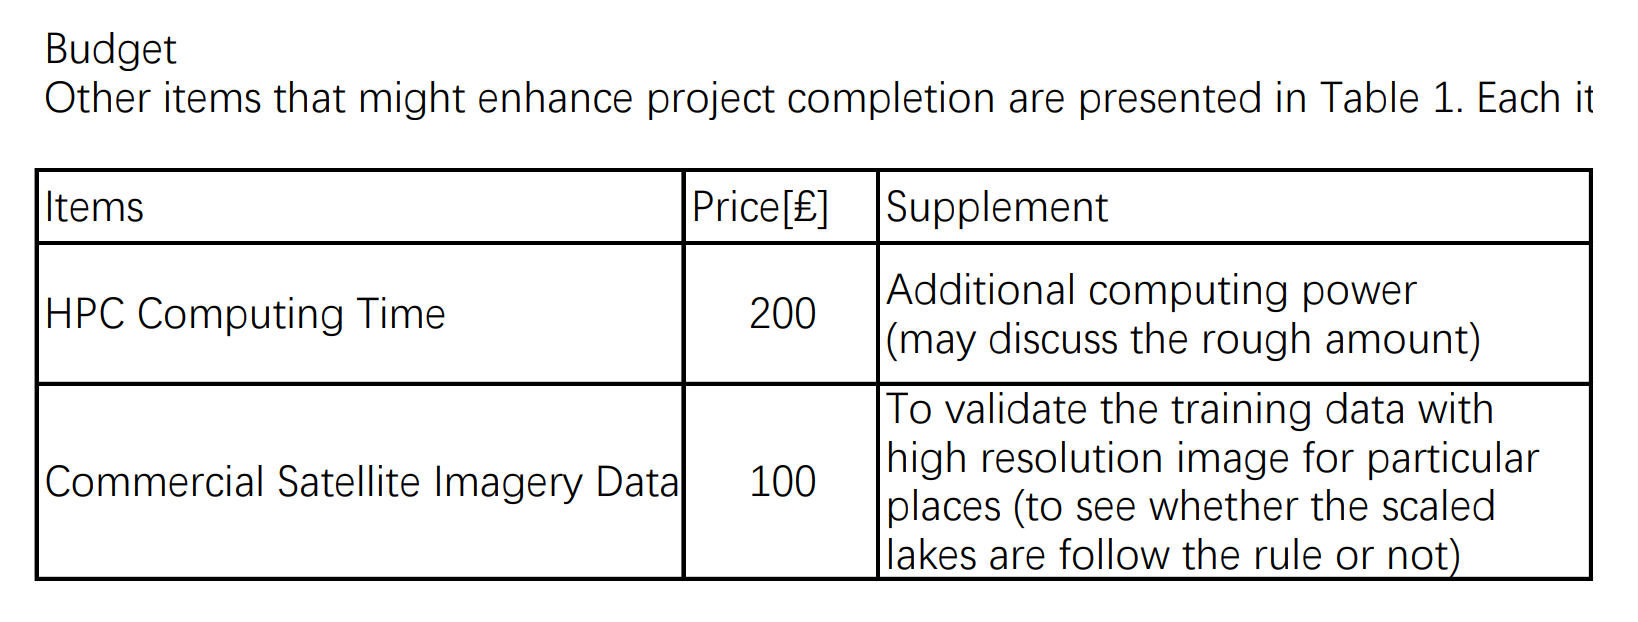
\includegraphics[scale=0.3]{introduction/Figure2.png}
    \caption{Budget}
    \label{Fig.2}
\end{figure}

\section{Supervisor Declaration}
\large{I have seen and approved the project and budget.}
\\
\large{Supervisor Signature:}     
\\
\large{Date:}


